%!TEX root = ..\..\dissertation.tex
\section{Brownfield Platform Development}\label{sec:brwnfld}
\cref{paper:CMS2019} is entitled \citetitle{SorensenCMS2019}, written for and presented at the 52nd CIRP Conference on Manufacturing Systems (CMS2019) in 2019.
It relates to and addresses \cref{resq3} by answering the follow sub-question:
\begin{enumerate}[leftmargin=3em]
  \item[RQ3.2] What steps should a manufacturer take to develop platforms of standardised assets based on existing manufacturing systems and environments?
\end{enumerate}
Through an evolving case study spanning multiple years, this paper presents seven recommended steps manufacturers can take to develop manufacturing system platforms based on an existing production landscape.
While greenfield approaches to development of platforms and changeable manufacturing exist, there are few explicit brownfield approaches manufacturers can use.
The brownfield approach presented in the following is intended to lower the barrier of entry for manufacturers looking to achieve changeable manufacturing.

\subsection{Extended Abstract}

\subsubsection*{Introduction \& Background}
Manufacturers looking to achieve changeable manufacturing in order to manage an increasing variety will often have existing product portfolios, manufacturing systems, and potentially platforms scattered throughout the company. 
This existing production landscape represents a large investment by the company, and is not something that can simply be scrapped for all new systems.
Rather than designing new changeable systems and products from scratch, considering and reusing elements of the existing production landscape could lower the barrier of entry for manufacturers looking to adopt changeable manufacturing.

Through greenfield approaches, systems are developed outside the constraints of prior work, existing systems, or ongoing projects.
\Gls{glos:platform} approaches typically do consider existing systems, but focus on development of new platforms, modules, and solutions~\parencite{JoergensenPaper,SorensenMCPC2017}.
Similarly, design of \gls{glos:RMS} and \gls{glos:CMS} usually employ greenfield approaches while still taking a manufacturer's requirements for \gls{glos:changeability} into account~\parencite{Andersen2017179,doi:10.1080/00207543.2017.1394594}.
Performing an internal evaluation of existing systems and their potential for change is, however, always recommended prior to or during design of \gls{glos:CMS}~\parencite{ElMaraghy2005}.

In contrast, through brownfield approaches systems are developed within the constraints of prior work, in this case, the existing production landscape.
Employing such an approach, platforms can be developed from existing solutions, essentially elevating them and preparing them for reuse rather than developing all new solutions and platforms.
To do so requires that the most likely \gls{glos:platformCand}s are identified, and as many of their characteristics as possible are standardised and documented, determining which characteristics may change, and which may not.
Thus, designers and developers can free up development time by solving frequent processes or functions with robust modules and equipment already present within the platform, allowing them to spend more time on less frequent tasks, new technologies, and efficiency improvements.

Manufacturing system \gls{glos:platform}s have an inherent connection with reconfigurable and changeable manufacturing, and while certain methods for \gls{glos:RMS} design do mention platforms, their role in the design of changeable manufacturing is rarely stated explicitly.
Based on the generic \gls{glos:RMS} design method by \textcite{Andersen2017179}, platforms are essentially applicable by and beneficial to designers during the later stages of the basic design phase (phase 3) and throughout the advanced design phase (phase 4).
The prior planning (phase 1) and task clarification (phase 2) phases set the scope and requirements for the design phase, while basic design (phase 3) use these to define system elements, interfaces, and modules for the system being designed.
In advanced design (phase 4), the concept from basic design is transformed into a detailed design representing the physical design and construction of the system.
Following the design phases, the system is implemented and subsequently operated and reconfigured as needed.
Having a platform consisting of standardised solutions with well-defined functions and interfaces could significantly ease the basic and advanced design phases.

\subsubsection*{Method}
The stage-gate approach presented in the following was developed as a result of an evolving case study, consisting of four consecutive platform projects, with an industrial partner.
Focus and the group of participants varied from project to project, with project one focusing on the nature, development, and utilisation of platforms, project two on the identification and documentation of platforms, project three on modelling and increasing the level of details, while project four is ongoing and focused on creating a framework and tools supporting platform development.
Additional details on the evolving case study and the four constituent projects are available in \parencite{SorensenAPMS2018}.

\subsubsection*{A Stage-Gate Approach}
The suggested brownfield \gls{glos:platform} development approach is a systematic stage-gate approach consisting of the seven stages listed below.
It is inspired by systematic design \parencite{Pahl2007}, going through the same four design phases, from planning and clarification (stage 1 and 2) to conceptual (stage 3), embodiment (4 and 5), and detail design (stage 6).
Stage 7, dealing with governance and maintenance of platforms, is outside these four basic phases of design, but is necessary for the continued life and function of \gls{glos:platform}s.
The seven stages are operational guidelines, and should generally be carried out in the listed order, although there is some need for flexibility in the approach.
It may also be necessary to complete multiple iterations of the approach for a satisfactory result.
\begin{enumerate}
  \item Assess changeability requirements
  \item Identify \gls{glos:platformCand}s
  \item Define essential functions
  \item Establish principal structure
  \item Define physical enablers
  \item Document platform
  \item Govern and maintain platforms
\end{enumerate}
Stages 1 and 2 are performed once per iteration, while stages 3--6 are performed for each identified platform candidate, and stage 7 continues throughout the entire life cycle of the platforms.
After each stage, the continued development of the relevant subject (\ie{} platform candidate) must be justified.
If no justification for continued development can be found, the remaining stages should be skipped and the decision regarding the platform candidate is noted for future reference.
Stages 1 and 7 are considered more related to an overarching platform framework than actual platform development.
Thus, this study focuses on stages 2--6, covering stages 1 and 7 only briefly.

%Assessment
A prerequisite for any development related to \gls{glos:changeability}, including platform development, is the assessment of a company's changeability requirement (stage 1).
This sets the scope for all subsequent stages of platform development by screening a company's need for changeability, determining change drivers, recommending type and degree of changeability, and estimating potential benefits.
One way to perform this assessment is through the participatory method proposed by \textcite{doi:10.1080/00207543.2017.1394594} considering existing products, manufacturing systems, and facilities, subsequently recommending a path to changeability to individual companies.

%Platform identification
Identification of \gls{glos:platformCand}s (stage 2) represents the identification of the essential functions, processes, equipment, or knowledge with the potential to become platforms.
Initially, existing manufacturing systems should be grouped and classified in order to create a map of a company's production landscape.
This should be done in a standardised way facilitating comparison and identification of commonality across the systems.
Group technology and classification coding is one example of how this can be achieved, although few coding schemes exist for manufacturing systems \parencite{ElMaraghy2006Complexity,elmaraghy2010classification}.
Decision algorithms and criteria can then be applied to the classified manufacturing systems, returning a recommendation of which processes or equipment should be investigated further based on the company's specific changeability requirements.
Each of the identified platforms should be further developed, either in individual projects or as part of projects intended to make use of the specific platform. 

%Essential functions
As essential functions are defined (stage 3), the function of a particular platform candidate becomes clear.
They are the functions a candidate must carry out for it to fulfil its purpose.
Standardising these functions means standardising the functional capability of a system.
Initially, top-level functions must be identified and subsequently broken down into sub-functions.
A function sequence should be used to represent each platform candidate, thus describing exactly what functions the platform candidate is supposed to perform.
Should a candidate be capable of carrying out multiple top-level functions, such as a robot capable of performing both material handling and assembly, a function sequence should be created for each.

%Principal structure
Establishing the principal structure (stage 4) of a platform candidate, refers to the creation of a structure describing the interactions between elements of a platform candidate and its environment; essentially a simple view of a \gls{glos:platformCand}'s architecture, illustrated on \cref{fig:principStruct}.
While \gls{glos:interaction}s and corresponding \gls{glos:interface}s are not fully specified at this stage, they should be identified and assigned a corresponding type, \ie{} spatial, energy, information, or material~\parencite{Pimmler94integrationanalysis}.
A close examination of existing physical instantiations of the platform candidate can help establish the principal structure.
On \cref{fig:principStruct}, the principal structure for a robot system is shown, with the robot itself consisting of a manipulator, control system, and a base.
The robot system further consists of an end effector connected to the robot's manipulator, and a number of supporting devices.
\begin{figure}[tb]
  \centering
  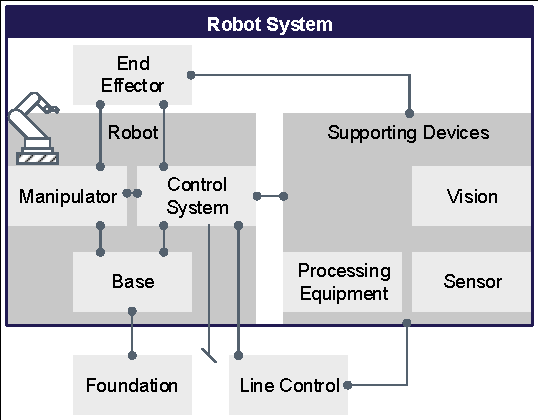
\includegraphics[width=.5\textwidth, trim=2 2 2 2, clip]{mainmatter/researchResults/figures/principStruct.pdf}
  \caption[Principal structure of a robot system.]
  {A robot, an end effector, and optional supporting devices form the principal structure of a robot system.
  The foundation and line control elements are outside the robot system.
  Adapted from~\parencite{SorensenCMS2019}.}\label{fig:principStruct}
\end{figure}

%Enablers
Defining the physical enablers (stage 5) for a platform candidate is essentially the act of selecting the future physical instantiations of a candidate.
It means specifying a few well-defined solutions spanning a range of applications, rather than creating or selecting a single solution to deal with all potential applications.
A variety of physical enablers are available for each element shown on \cref{fig:principStruct}.
To distinguish enablers and select an appropriate one for a given application, a set of requirements must be defined for all enablers, forming a basis for comparison and selection.
These could be \eg{} accuracy, reach, and load for the robot on \cref{fig:principStruct}.
Such requirements can then be used to form areas of application, under which each existing enabler can be grouped.
A decision can then be made, based on the performance and characteristics of enablers, on which enablers should continue to exist and be used within a given area of application.
All enablers, whose continued existence is justified, have their principal structure detailed into a physical structure, including further specification of elements, interfaces, and interactions.

%Documentation
Platform documentation (stage 6) is a crucial yet oft-overlooked part of platforms.
They are necessary for \gls{glos:platform}s to be widely adopted within a company.
The documentation for a platform should include all requirements, models, decisions, reasoning, \etc{} from the previous stages, and make them accessible to relevant stakeholders.
ISO 42010, providing a standard for architecture descriptions, presents a way to accomplish this and customise the documentation to specific stakeholder concerns~\parencite{ISO42010}.
Some recommended sections of the platform documentation are: (a) vocabulary, (b) scope, (c) requirements, (d) essential functions, (e) principal structure, (f) physical enablers and interfaces, (g) detailed enablers, and (h) further reading.

%Governance
Platform governance and maintenance (stage 7) is the infrastructure in a company facilitating the continued use of platforms. 
Use of \gls{glos:platform}s in a company requires commitment from all levels of the company; both the goal of using them as well as their existence must be clear at all levels of the organisation.
Responsibilities and procedures to be followed should be set and become an integral part of new development projects.
Information on the platforms themselves must be easily available to all who need the information.
Platforms must also regularly be maintained, ensuring that the design, decisions, and reasoning from previous iterations still hold, redesigning or scrapping the platform if needed.
Emerging technologies or changing requirements must be considered in this process.
Stage 7 does not truly end as long as a company is committed to using platforms.

\subsubsection*{Conclusions}
The stage-gate approach for brownfield \gls{glos:platform} development presented above outlines seven stages to the platform development process.
These stages take companies through an assessment of changeability requirements, through identification of platform candidates and development of these, to the documentation and governance of the final platform.
It is an alternative to the more prevalent greenfield approaches in the field of platform development, as it bases development on a company's existing production landscape, potentially speeding up the design and implementation of changeable manufacturing.
Can no suitable brownfield solution be found, a greenfield approach can be employed to develop a new solution.

\subsection{Implications}
In the study presented above, an attempt at transitioning from greenfield to brownfield development of \gls{glos:platform}s have been made.
It describes a number of generic recommendations for companies to follow on their path to changeable manufacturing through platforms, building on the experiences and challenges faced during the evolving case study~\parencite{SorensenAPMS2018}.
The seven stages are operational guidelines in a recommended order of execution, but there is room for flexibility.
Certain steps can be skipped or saved for later, if the need arises.
As with any generic approach, some tailoring to the individual company is to be expected, since differences in circumstances, environment, and organisational structure \etc{} will play a part in the tools and approaches a company should utilise.
The outcome of the paper can be summarised as follows:
\begin{enumerate}
  \item A stage-gate approach to brownfield platform development.
  \item Potentially a lowered barrier of entry for designing and implementing changeable manufacturing through platforms.
  \item Recommendations for how to approach certain aspects of platform utilisation related to documentation, governance, and maintenance.
\end{enumerate}